\begin{figure}[H]
    \begin{center}
        \includegraphics*[scale=0.5]{images/1.png}
        \caption{\label{figure 1} Schéma d'un montage avec une diode, une résistance $R=270 \Omega$ et un GBF.}
    \end{center}
\end{figure}

Nous avons réalisé le montage précédent et avons ensuite mesuré la tension aux bornes de la diode, de la résistance et avons estimer en conséquence le courant du circuit en variant la tension d'entrée. Nous avons obtenu les résultats suivants :

\begin{table}[H]
    \centering
    \begin{tabular}{|c|c|c|c|c|c|c|c|c|c|c|c|c|}
        \hline
        $E$ (V) & -5 & -4 & -3 & -2 & -1 & 0 & 1 & 2 & 3 & 4 & 5\\
        \hline
        $V_D$ (V) & -5 & -4 & -3 & -2 & -1 & 0 & 0.63 & 0.69 & 0.72 & 0.74 & 0.77\\
        \hline
        $V_R$ (V)& 0 & 0 & 0 & 0 & 0 & 0 & 0.37 & 1.34 & 2.22 & 3.22 & 4.2\\
        \hline
        $I$ (mA) & 0 & 0 & 0 & 0 & 0 & 0 & 1.3 & 4.6 & 8.13 & 11.9 & 15.49\\
        \hline
    \end{tabular}
    \caption{\label{table 1} Tableau correspondant aux mesures de la figure \ref{figure 1}.}
\end{table}

\newpage
Voici ensuite la courbe représentant l'intensité du courant I en fonction de la tension $V_D$ : 

\begin{figure}[H]
    \begin{center}
    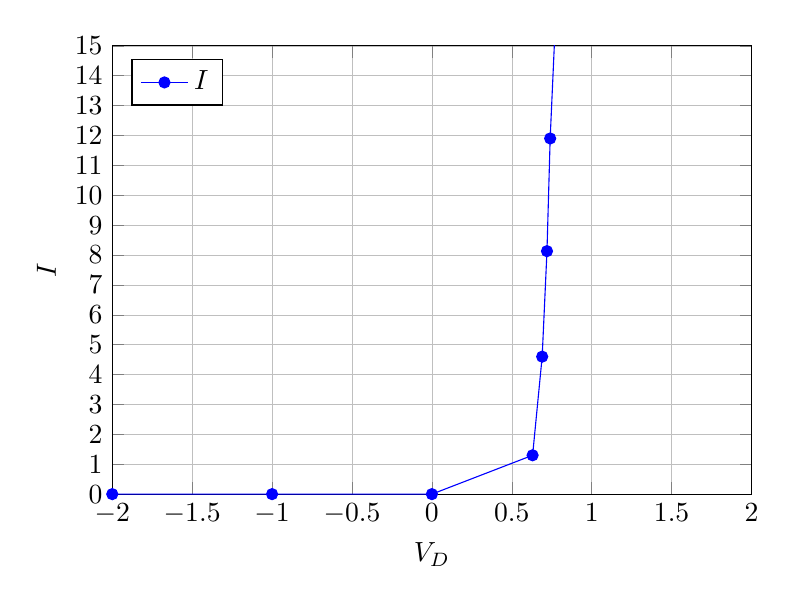
\begin{tikzpicture}
        \begin{axis}[
            xlabel={$V_D$},
            ylabel={$I$},
            xmin=-2,
            xmax=2,
            ymin=0,
            ymax=15,
            grid=both,
            grid style={line width=0.2pt, draw=gray!50},
            width=0.8\textwidth,
            height=0.6\textwidth,
            legend pos=north west,
            legend cell align={left},
            ytick distance=1, % Set the y-axis tick distance to 1
        ]
        
        % Plot the curv
        \addplot[blue, mark=*] coordinates {
            (-5, 0)
            (-4, 0)
            (-3, 0)
            (-2, 0)
            (-1, 0)
            (0, 0)
            (0.63, 1.3)
            (0.69, 4.6)
            (0.72, 8.13)
            (0.74, 11.9)
            (0.77, 15.49)
        };
        \addlegendentry{$I$}
        
        \end{axis}
    \end{tikzpicture}
    \caption{\label{graph 1} Courbe représentant l'intensité du courant I en fonction de la tension $V_D$.}
    \end{center}
\end{figure}

Nous pouvons distinguer deux états distincts qui sont : 

- Si la tension est négative, alors le courant est nul donc la diode est dite \underline{"bloquante"}

- Si la tension est positive, alors le courant est non nul donc la diode est dite \underline{"passante"}\\


La résistance dans ce circuit permet de simuler la résistance de la diode lorsque la tension est négative et que la diode soit "bloquante".